\subsection{Constraints on the dark energy}
With the Pantheon dataset, the matter density of the flat $\Lambda$CDM model is constrained to be $\Omega_M=0.278 \pm 0.007$. With 24 long GRBs alone, the matter density is constrained to be $\Omega_M=0.307 \pm 0.065$. It indicates that the Hubble diagram in high redshift is consistent with the $\Lambda$CDM model
\begin{figure}[h]
	\centering
	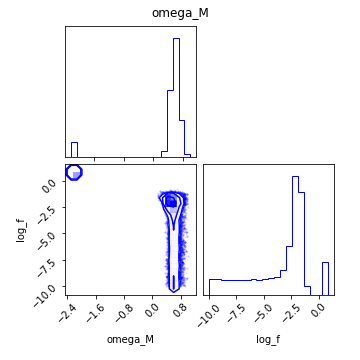
\includegraphics[width=\textwidth]{pantheon/gp/18_omega_M_corner_plot.png}
	\caption{GRB Hubble Diagram}
	\label{fig:OmegaM_GP}
\end{figure}

